
\section{FLARE}
\label{sec:system}
\vspace{-.2cm}
% 	\par In this section we introduce FLARE, a system to enable flexible sharing 
%     of GPUs between LC and BE applications to improve hardware utilization. 
    %The purpose of spatial sharing among applications is to improve GPU resource utilization.
    %In addition, FLARE dynamically selects configurations to improve resource utilization. 
    %Furthermore, FLARE
    %dynamically explores the configuration space and 
    %searches for the best configuration, which satisfies the QoS requirement and in the meantime 
    %the overall co-run throughput of the pair is maximized.
	
	%\subsection{Goals}
	%	\par The primary design goal of FLARE is to maximize the overall throughput 
    %    of a co-run pair subject to QoS constraints on LC applications. 
    %    Datacenters often co-locate applications on shared servers to 
    %    improve resource utilization. But GPUs lack the fine-grained context switching 
    %    and preemption features of CPUs, making sharing them more difficult. 
    %    On shared GPUs, FLARE improves hardware utilization by safely sharing 
    %    the GPU between BE and LC applications.
%		\par FLARE is designed to consider the trade-offs between 
    %    latency and throughput caused by different co-run configurations. 
    %    The system must configure co-runs to maximize the available throughput 
    %    while respecting QoS requirements. This needs to be done quickly, 
    %    with as few QoS violations along the way as possible. 
    %    Resource allocation occurs at the kernel level, 
    %    so the dynamic reconfiguration can only happen between runs.
	
	\subsection{System Overview}
		The goal of FLARE is to enable flexible sharing between LC and BE applications 
        and optimize resource partitioning 
        to enforce QoS as well as maximize overall throughput 
        of co-run pairs. %FLARE implements spatial sharing through Hyper-Q technique.
        FLARE addresses the trade-off between latency and throughput 
        based on offline and online dynamic search algorithms to quickly figure out an optimized co-running configuration. The system, as shown in Fig.~\ref{fig:system}, consists of the following three components: \\%Kernel Transformation, Initial Configuration Selection, and Online Refinement.\\
		\textbf{\textit{Kernel Transformation}} FLARE transforms the BE application 
        to allow it to yield an arbitrary number of thread blocks on each SM. 
        Note that we assume there is no access to the kernels of LC applications 
        submitted by users, so FLARE does not transform the kernels of LC applications.\\
		 \textbf{\textit{Initial Configuration Selection}} To address the problem of unavailable LC applications for offline profiling, FLARE co-runs pairs of diverse microbenchmarks with many resource sharing configurations to characterize the performance degradation space. Based on the characterization, when the LC application arrives, FLARE only profiles its kernel invocation once to quickly model the performance degradation for both the LC and BE applications. FLARE then selects an initial configuration to spatially co-run the applications. \\
		\textbf{\textit{Online Refinement}} During the co-running, FLARE collects the performance degradation timing data as feedback to dynamically adapt the next configuration to use. By using the co-run degradation data of microbenchmarks, FLARE intelligently skips configurations and quickly reaches the optimal configuration to use for spatial co-running.
		%Each new kernel needs to be transformed to support spatial sharing and benchmarked for a single run with NVIDIA's Cuda profiler $nvprof$ before it is ready to run. The profiling results are used to characterize the expected behavior of the kernel when co-running to select an initial configuration, then an iterative process refines that configuration online. Each QoS kernel has a deadline $T_{dl}$ which is at least as long as the solo runtime $T_{solo}$. As long as that deadline is met, the configuration is satisfactory and the only other concern is how much throughput the configuration can achieve.
\subsection{Kernel Transformation:
				Enabling Spatial Sharing}


%\vspace{-0.8cm}
\begin{wrapfigure}{l}{0.5\textwidth}
		\centering
		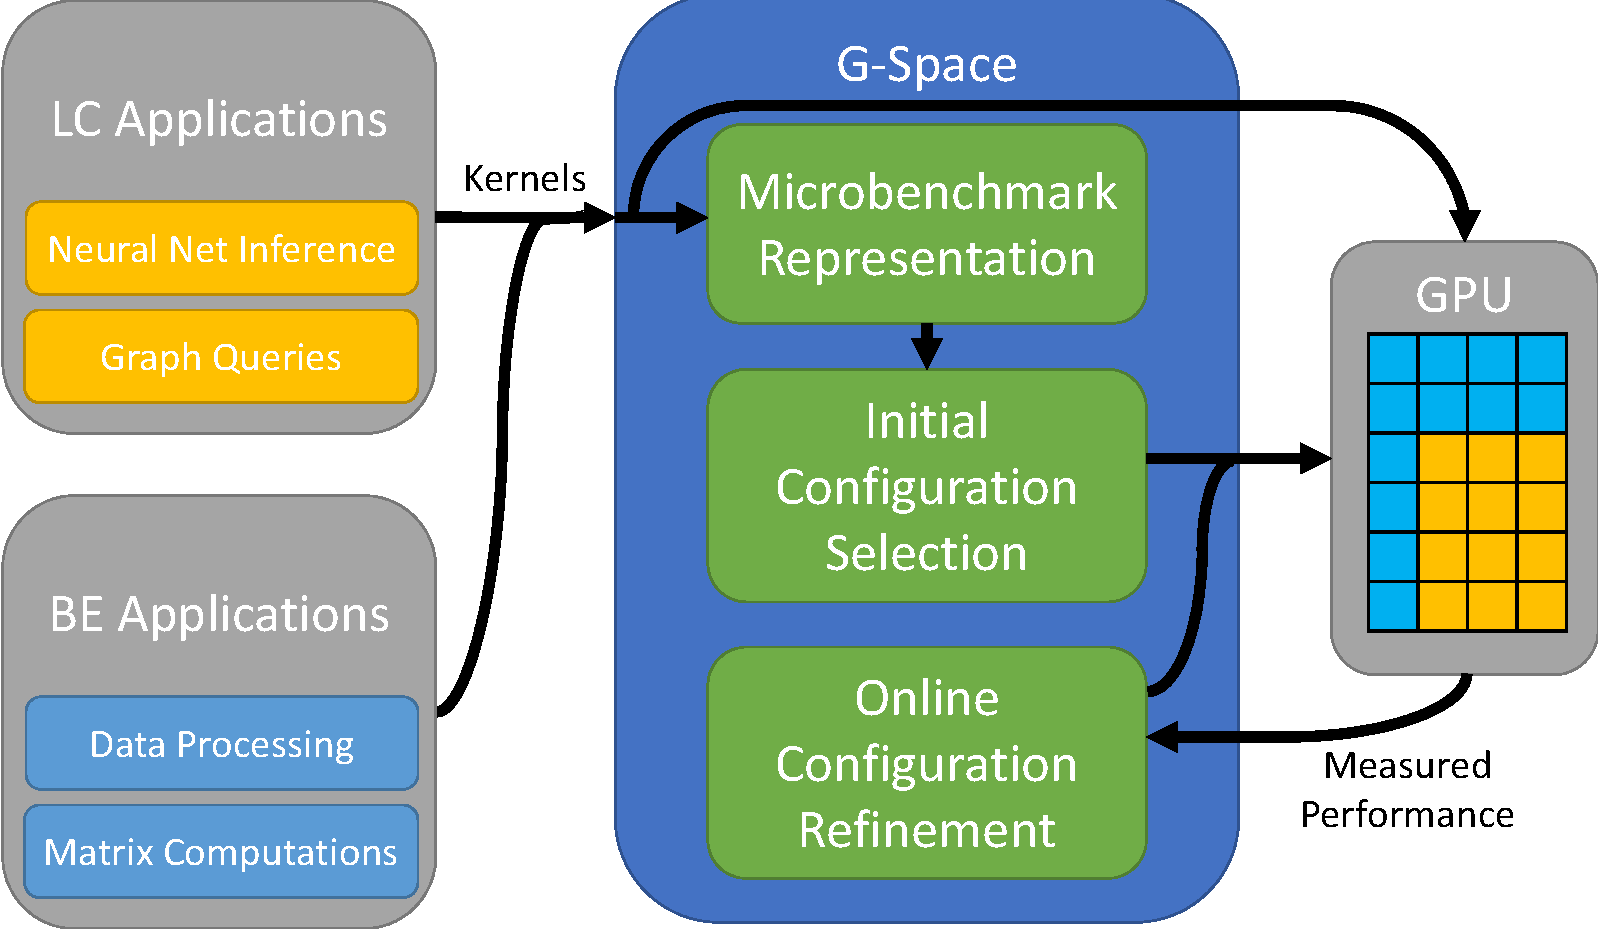
\includegraphics[width=\linewidth]{figures/system_diagram_cropped.pdf}
		\caption{The FLARE System}
		\label{fig:system}
		\vspace{-.2in}
		\end{wrapfigure}
		Kernel transformation enables the BE application to yield resources when a LC application is scheduled to the same GPU. The design, inspired by SM-centric transformation~\cite{Wu+:ICS15} and FLEP~\cite{Wu:ASPLOS2017}, runs just enough thread blocks to occupy the whole GPU. Specifically, given that a GPU has $N$ SMs and each SM runs up to $K$ thread blocks, FLARE schedules $N \times K$ thread blocks, each running the algorithm described in Fig.~\ref{fig:alg1}. Every thread block first invokes $get\_sm\_id()$ to obtain the ID of the host SM and then $atomic\_get\_blk\_id()$ to get its unique block ID on that SM, starting from 0. Each thread block stays in a while loop as long as there are tasks left to execute. At the beginning of each iteration, each thread block gets a unique ID. If a thread block ID is larger than the specified value $num\_blks[sm\_id]$, which is set by CPU, it means that the thread block needs to be yielded. To control the spinning overhead, we follow the approached proposed in~\cite{Wu:ASPLOS2017} to control the granularity of the tasks. Once the resource of the yielded thread blocks is released, the kernel of the LC application can acquire the resource and start co-running. After the LC application is finished, the BE application is notified and launches the same number of thread blocks as yielded to fully occupy the GPU again. 
		

		Although the algorithm enables arbitrary ways to yield thread blocks, it requires the CPU and GPU to share the array $num\_blks$, containing $num\_SMs$ elements, which may incur non-trivial communication overhead when $num\_SMs$ is large for high-end GPUs. To address this problem, FLARE uses the algorithm shown in Fig.~\ref{fig:alg2} to sacrifice flexibility for reduced overhead. In this new design, FLARE asks the BE kernel to yield the same number of thread blocks (i.e., $k$) on a subset of SMs (i.e., $n$). Since thread blocks of a kernel have similar behaviors and the SMs are homogeneous, we expect this simplified design to perform as well as the more flexible one.

		
		%The result of 
% 		This mechanism is summarized in the following workflow. 
%         %\begin{enumerate}
% 		%	\item 
% 			BE application claims all the resources on a GPU using exactly the same threads supported on the GPU;
% 		%	\item 
% 			When a LC application arrives, BE kernel yields resources;
% 		%	\item 
% 			The LC kernel greedily uses all yielded resources;
% 		%	\item 
% 			The BE application reclaims resources once LC kernel completes.
%			\begin{minipage}{0.48\linewidth}
%\begin{algorithm}[H]
%\caption{Arbitrary thread block yielding.}
%\tcp{Run by each thread block of BE kernel}
%\tcp{Global array num\_blks[num\_SMs]}
%\begin{algorithmic}
%\label{alg:alg1}
%\Function{BE\_Kernel}{$\cdots$} 
%  \State sm\_id = get\_sm\_id()\;
%  \State blk\_id = atomic\_get\_blk\_id()\;
%  \While{task\_queue is non-empty} {
%    \eIf{ blk\_id $>$ num\_blks[sm\_id]}{ quit\;
%    }{ 
%      \State task = pull\_task()\;
%      \State execute(task)\;
%    } 
%  } 
%\EndFunction
%\end{algorithmic}
%\end{algorithm}
%\end{minipage}
%\hfill
%\begin{minipage}{0.48\linewidth}
%\begin{algorithm}[H]
%\caption{Less exible thread block yielding to reduce overhead.} 
%\tcp{n: number of SMs to yield blocks}
%\tcp{k: number of blocks to yield}
%\begin{algorithmic}
%\label{alg:alg2}
%\Function{BE\_Kernel}{$\cdots$} 
%  \State sm\_id = get\_sm\_id()\;
%  \State blk\_id = atomic\_get\_blk\_id()\;
%  \While{task\_queue is non-empty} {
%    \eIf{ sm\_id $<$ n \textbf{and} blk\_id $>$ num\_blks[sm\_id]}{ quit\;
%    }{ 
%      \State task = pull\_task()\;
%      \State execute(task)\;
%    } 
%  } 
%  \EndFunction
%\end{algorithmic}
%cudaMalloc((void**)&num\_blks, sizeof(int)*num\_SMs)
%\end{algorithm}
%\end{minipage}
		%\end{enumerate}
		%\par By this mechanism, a particular number of blocks can be scheduled to each SM, so each kernel will have partial, simultaneous access to the GPU, enabling a spatial co-run. The allocations used by this paper will use a rectangular allocation of resources to the QoS kernel (k blocks on each of n SMs), and the rest of the GPU for the throughput kernel. Blocks running on the same SM will contend for that SM's computation resources and L1 cache space. All blocks on the GPU contend for the L2 cache space, main memory bandwidth, and PCIe bandwidth.
%\begin{wrapfigure}{l}{0.7\textwidth}
\begin{figure}
\vspace{-.2in}
\begin{center}
\begin{subfigure}[b]{0.3\textwidth}
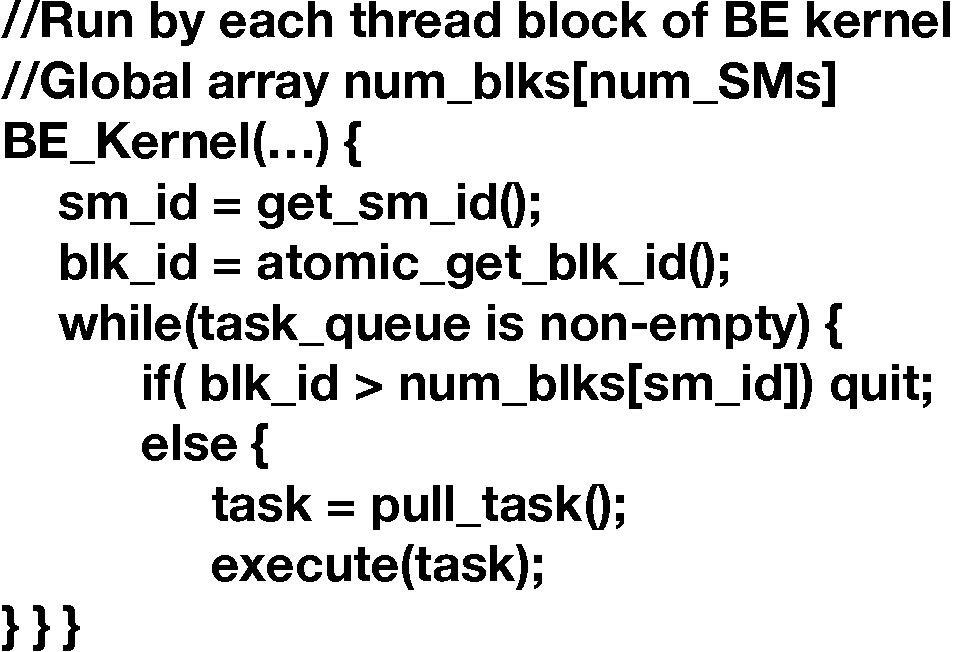
\includegraphics[width=\linewidth]{figures/trans_1-crop.pdf}
\caption{Arbitrary thread block yielding.}
\label{fig:alg1}
\end{subfigure}
\begin{subfigure}[b]{0.4\textwidth}
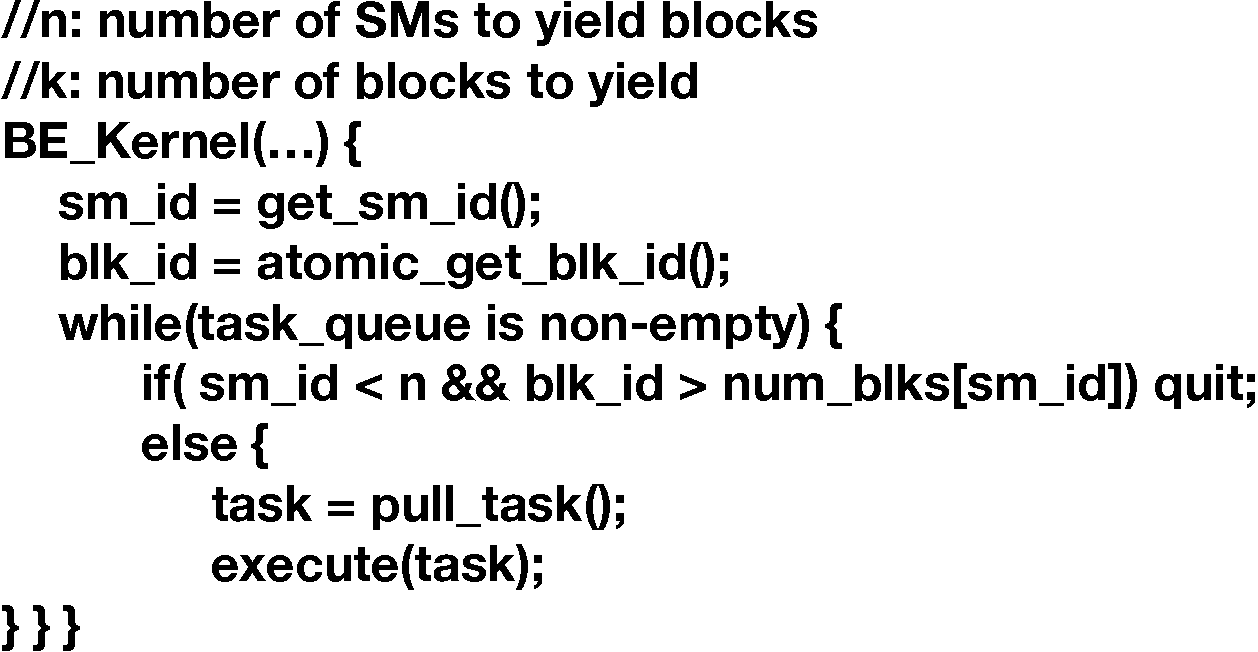
\includegraphics[width=\linewidth]{figures/trans_2-crop.pdf}
\caption{Less flexible thread block yielding to reduce overhead.}
\label{fig:alg2}
\end{subfigure}
\end{center}
\caption{Transformed BE kernels to allow spatial co-run.}
\vspace{-.5in}
\end{figure}
%\end{wrapfigure}
\subsection{Initial Configuration Selection:
				Microbenchmark Driven}
				\label{sec:initial}
		Due to the large spectrum of LC applications, FLARE cannot exhaustively profile BE-LC co-run pairs to find the optimal configuration. Instead, FLARE estimates the performance of BE-LC co-runs using microbenchmarks. Each kernel is matched with microbenchmark configurations that best represent its solo-run profiling statistics. Designing microbenchmarks  that represent real-world applications is not easy, because the performance of a kernel is affected by many factors and the importance of each factor varies for different kernels. But the relevant features should be those related to resources for which the kernels contend when co-running. Out of the 120 performance counters of NVIDIA's $nvprof$ profiler, we select the following 7 metrics which reflect or affect resource contention:
		%\begin{itemize}
		%	\item 
			L1, L2 cache hit rate,
		%	\item 
			DRAM, L2, and L1 bandwidth utilization,
		%	\item 
			arithmetic intensity, 
		%	\item 
			and total number of instructions. 
		%\end{itemize}
        
		To produce microbenchmark instances with varied features, we design a parameterized 
        kernel with two parts. The first part loads a 1-D array and the second part 
        contains a loop that performs pure arithmetic operations on the loaded data in each iteration. 
        %Note that it is quite difficult to decouple the parameters used in micro-benchmarks to simulate metrics related to $L1$ and $L2$ cache.
        %Hence, the 
        The microbenchmarks use the following 4 parameters to sample the configuration space: {\em stride length} to specify the distance between memory accesses from adjacent threads and hence control spatial locality of each thread block, {\em overlap ratio} to specifying the overlap between working sets of adjacent warps, {\em iterations} to control arithmetic intensity by specifying the number of iterations of the loop and {\em the number of threads} to run in total.
		
	    With 9 different stride lengths from 0 to 128 elements (L2 cache line size), 5 different overlap ratios ranging from 0 to 0.2, 
        iteration counts from 1 to 4, and a fixed number 160K of threads, 
        there are 180 different configurations of the microbenchmark. 
        We find that the range of these metrics covers most real world applications by tuning these parameters.
     
        %above, 
         %The range of L1 hit rate of microbenchmarks is $\left[4\%, 60\% \right]$ 
        %and L1 hit rate of real world application is from $0.22\%$ to $64\%$. This rate can be further increased if we tune up the overlap ratio. 
        %The current value is large enough for our experiments.
        %L1 hit rate of our microbenchmarks almost cover the range of real world application. 
        %It has been confirmed by the profiling data that the stride length affects 
        %the hit rates. 
         %We find that microbenchmark arithmetic intensity falls 
        %between $\left[50\%, 98\%\right]$. The minimum value of arithmetic intensity is $50\%$ where all the instructions in the kernel are memory operation. 
        %Although the theoretical maximum value is $100\%$, this kind of application is useless. 
        
        %Each %one of these 
        %Instance is run under $nvprof$ to 
        %characterize its performance according to the 7 parameters above. 
        Running all pairs of these microbenchmarks on all possible co-run configurations gives a large input dataset for training models 
        to get a sense of the patterns that arise. %We evaluate two low-latency techniques for utilizing this dataset to predict performance degradation of application kernels. \\
%\begin{algorithm}[!ht]
%\caption{Microbenchmark pseudocode}
%\begin{algorithmic}
%\label{alg:micro}
%\Function{microbench}{data, stride, overlap, arithmetic}
%\State get\_block\_id()\;
%\State get\_warp\_id()\;
%\State calculate\_warp\_offset()\;
%\State i = 0\;
%\While{i less than arithmetic}{
%  \State pure\_arithmetic\_operations\;
%  \State i++\;
%}
%\EndFunction
%\end{algorithmic}
%\end{algorithm}
		Given 180 different instances of the microbenchmark, we co-run each pair of them 
        in all possible ways to spatially share the GPU, resulting in a total of $640 \times 640 $ co-runs. 
        %Note that the total is not half of that, because we need to use each instance to represent a BE workload and a LC workload. 
        %Each co-run has two sets of characterization features for the two micro-benchmark instances, respectively, 
        %a co-run configuration for resource partitioning, and the corresponding performance degradation data. 
        Based on these results, FLARE has the following two methods to select the initial configuration. \\
%\vspace{.2cm}	
\textbf{\textit{Linear Regression}} %The linear regression method builds a
%pair of models to predict the performance degradation for each of the two co-running kernels.
%Linear model have the same set of features: 14 profiled features from the two co-running
The linear model has 16 features: 14 profile features from two
microbenchmark instances and the SM configuration (i.e., $n$ and $k$ in Fig.~\ref{fig:alg2}). 
%The model, therefore, concatenates the two 7-element
%feature vectors and 2-element configuration vector into a single 16-element
%vector. 
The linear regression maps that 16-element vector onto the
1-dimensional output space describing either estimated latency or throughput.
FLARE uses all the data from the offline co-runs as training data to build the
linear regression model. % (i.e., training the weights). %After deployment, 
 FLARE profiles 
one iteration of a solo-run of the BE kernel and the LC kernel (when it becomes available) to obtain the 14
characterization features and combine them with the other two features to get the feature vector of co-run applications. Then FLARE uses the linear regression models to
estimate the co-run performance degradation given each of the co-run
configurations, and finally selects the one that satisfies QoS and maximizes throughput.
Since the linear models are quite lightweight, the initial configuration-selection based on this method has a trivial overhead.\\
%\vspace{.2cm}
\begin{wrapfigure}{l}{0.5\textwidth}
			\centering
			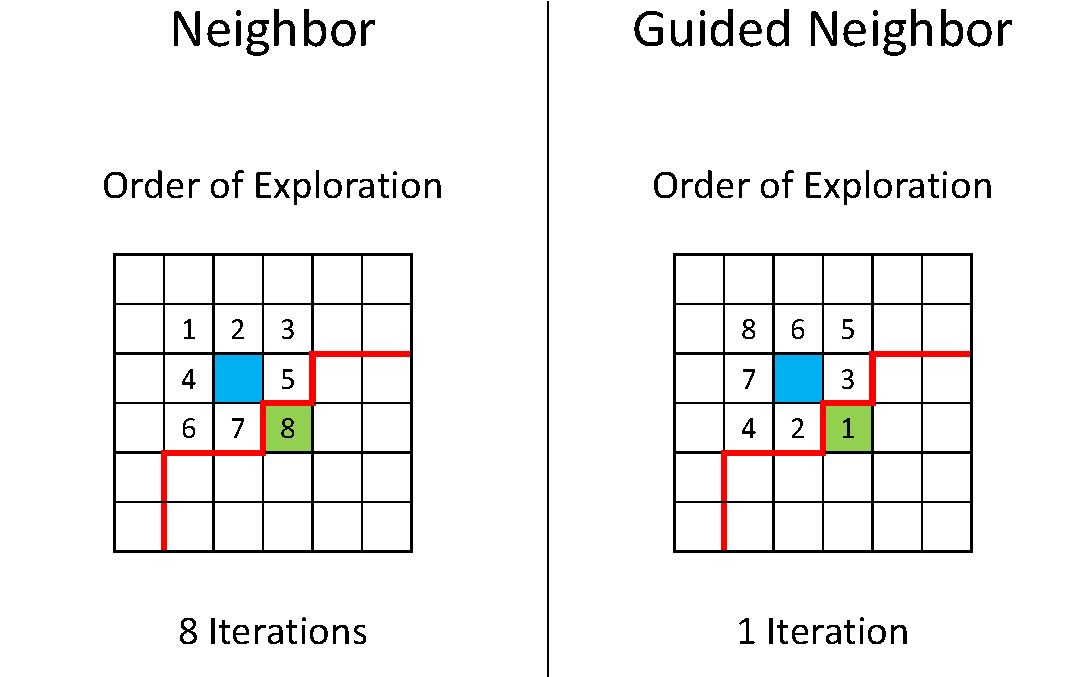
\includegraphics[width=\linewidth]{figures/new_search.pdf}
			\caption{Online search methods.}
			\label{fig:search}
			\vspace{-.3in}
			\end{wrapfigure}
		\textbf{\textit{Nearest Neighbor}} Like the linear regression method, the nearest neighbor method also profiles 
        one iteration of the BE and LC kernels to obtain their characterization features. For each kernel, 
        it then searches for a profiling characterization feature vector among the microbenchmarks that is the most similar 
        to that kernel in Euclidean distance. Specifically, each value of the 7-element feature vectors is normalized 
        to the range (0,1), and this method searches for the nearest microbenchmark feature vector $\vec{b}$ to the 
        feature vector of the real benchmark $\vec{m}$. 
        The nearest neighbor method selects the microbenchmark for which the quantity $\| \vec{m} - \vec{b} \|_2$ is minimized. 
        Each pair of representatives has offline-generated performance results on all of the co-run configurations available, 
        so this gives another estimate of the performance degradation across the configuration space. 
        Based on this, FLARE selects the configuration that satisfies QoS and maximizes throughput. This method requires no training and incurs negligible runtime overhead.
	\subsection{Online Refinement: Dynamic Reconfiguration}
%		\begin{figure}
%			\centering
%			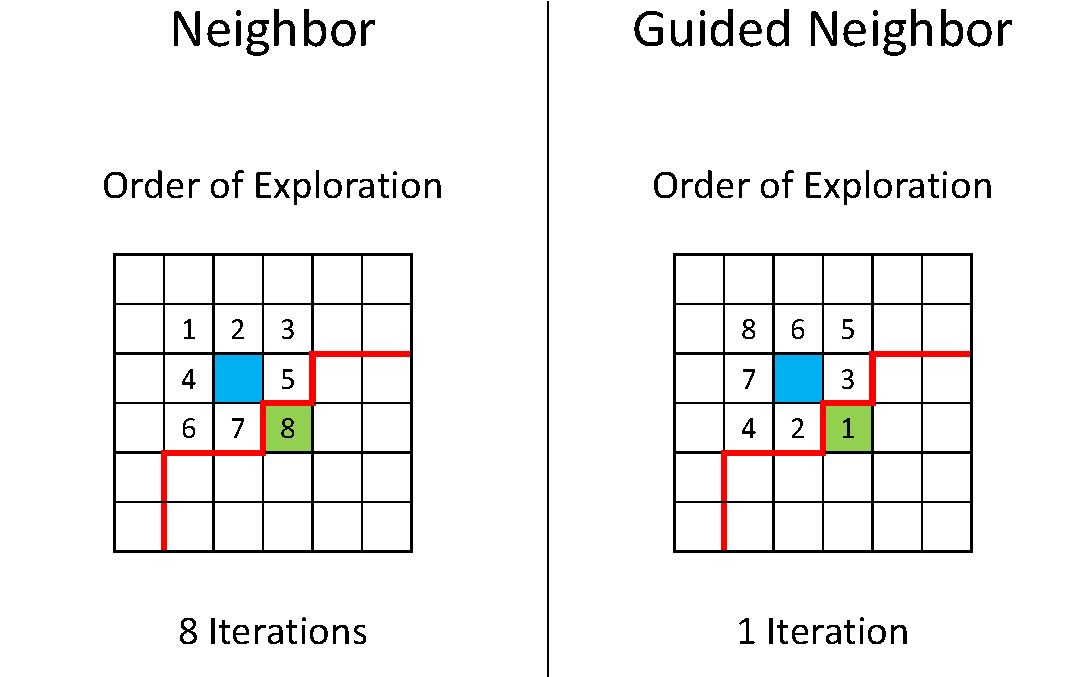
\includegraphics[width=8cm]{figures/new_search.pdf}
%			\caption{Online search methods.}
%			\label{fig:search}
			%\vspace{-0.8cm}
%		\end{figure}
The final configuration we select should be one with the highest possible throughput while still satisfying QoS. The initial configurations produced by the previously discussed methods are unlikely to match the globally optimal result every time. Therefore, configurations will need further refinement based on real performance feedback as shown in Fig. \ref{fig:system}. %In other words, FLARE needs to try a subset of configurations (i.e., execute the co-running kernels given those configurations) to figure out the optimal one. When FLARE tries a configuration, we say that configuration is explored. Note that due to the smooth performance degradation shown in Figure~\ref{fig:corun-scalability}, it may seem that a binary search-based approach can minimize the number of explored configurations. However, it does not directly translate to minimized search time. For example, exploring the extreme configuration of allocating most resources to the BE kernel may lead to unacceptable QoS violation for the LC kernel. So not only should these approaches find the optimal configuration, they should do it quickly and with as few QoS violations as possible. To achieve this goal, 
FLARE starts at the initial configuration and gradually explores the neighborhood to finally reach the optimal configuration. FLARE includes two approaches to performing the search as follows.\\
%\vspace{.2cm}
\textbf{\textit{Neighbor Search}} We demonstrate the idea of the first approach pictorially in Fig.~\ref{fig:search} (left panel). The cells represent configurations. Towards the bottom left corner, the configurations give more resources to the LC kernel. %Therefore, there should exist a continuous region of cells (included by the red line) that can satisfy the QoS requirement. 
The search process starts with an anchor cell (colored in blue), which should initially correspond to the configuration returned by the process described in Section~\ref{sec:initial}. It then explores all the 8 neighbor cells (the numbers show the order of the exploration), %which have not been tested before, 
and selects the best as the new anchor cell for the next round. Here the meaning of best is double-folded. When QoS is met, the best means that the overall throughput is optimal around neighbors. Otherwise, the best stands for the steepest decent of LC performance. This repeats until arriving at a cell where QoS is met and its throughput is the highest around its neighbors. \\
%The ``best'' neighbor configuration has different meanings when the anchor cell falls in the two different regions. In the regions of configuration that cannot satisfy the QoS, the best neighbor configuration is the one that minimizes the execution time of the LC kernel. Otherwise, the best neighbor configuration should minimize the execution time of the BE kernel. Therefore, when the initial configuration cannot satisfy the QoS, this approach tries to quickly enter the region that can satisfy the QoS and then maximize overall GPU utilization. This process works best on relatively low-noise data with a smooth performance degradation due to fewer allocated resources. It almost always eventually finds a configuration which satisfies QoS with better throughput than its neighbors, but may take many iterations to do so. To improve on this, it is important to maintain the same properties, but cut down on the total time taken. \\
%\vspace{.2cm}
\textbf{\textit{Guided Neighbor Search}} %With access to representative data from the micro-benchmarks, the patterns of the micro-benchmark and real kernel performance should be similar, even if not identical. This affords the opportunity to give some direction to the naive approach of the basic neighbor search. 
While the previous approach explores its neighborhood exhaustively, this approach searches first in the direction suggested by the microbenchmark data. Each neighbor cell has corresponding microbenchmark data, and therefore estimated QoS and throughput values associated with it. This gives some order to the neighbors in terms of their expected configuration performance, and we can simply explore the one with the best estimated performance. For example, Fig.~\ref{fig:search} (right panel) shows that according to the microbenchmark data, the bottom right neighbor configuration (labeled by 1) should produce the highest performance for the LC kernel. We then explore that configuration and select it as the anchor for the next round. By leveraging the microbenchmark data, we substantially decrease the number of steps required to converge. This process continues until it reaches a configuration where the QoS requirement of LC is satisfied and microbenchmark throughput is maximized. %, but have no guarantee of finding a higher quality configuration than the plain neighbor search, because the characterized performance degradation based on micro-benchmarks may not match that of the real applications. Hence, once the guided neighbor search terminates, we start a local refinement process to use the neighbor search process to improve QoS of the finally selected configuration.
%\vspace{.2cm}
%\textbf{\textit{Scalar Refinement Search}} The neighbor searches described above perform well when the initial configuration is close to the optimal configuration. Additionally, the guided search requires that the performance degradation pattern of the micro-benchmark exactly matches that of the application kernels. While we observe that the patterns are similar, the rate of degradation can differ significantly from the true pattern. We propose a hypothesis: that the micro-benchmark and application kernel performance degradation differences are equivalent to a multiplicative scalar difference in the QoS target. The red lines in Figure \ref{fig:corun-scalability} which separate configurations satisfying QoS from those that don't has an equivalent in the micro-benchmark space. The corresponding line in micro-benchmark space is typically substantially offset from the line that appears in that figure. For example, in the mm and lbm co-run there are 48 configurations which satisfy QoS with a QoS ratio of 2.0 (i.e., the QoS target is twice its solo execution time). Their representative micro-benchmark pair has 134 configurations which satisfy QoS for the same ratio, so the line is substantially offset toward the bottom-left. A similar line could be found by decreasing the QoS ratio used for the micro-benchmark. Scalar Refinement method can automatically perform this correction for the offset in an online fashion.
%This approach also starts at the configuration that was optimal for the micro-benchmark. Based on the performance data for that single run, we can adjust the micro-benchmark QoS ratio to better fit that result. If the result fails to satisfy QoS, the ratio needs to decrease to make it more restrictive as shown in Figure \ref{fig:search} (right panel). If it satisfies QoS by a wide margin, the ratio should increase to allow for a more aggressive configuration. Recomputing the micro-benchmark optimal configuration may give a new configuration, which we explore in the next iteration. This continues until the new and old configurations match, which happens very quickly. Figure \ref{fig:search} illustrates this process in terms of the line adjustment it implies. More precisely, scalar refinement adjusts the scalar $\gamma$ on the target QoS ratio $q$ for the micro-benchmark, such that the micro-benchmark search looks for configurations that satisfy a QoS ratio of $q \times \gamma$, with $\gamma$ initially 1. In subsequent iterations, if the real performance result exceeds the QoS target by a factor of $c$, then for the next iteration $\gamma$ will be decreased by an amount proportional to $c$. Conversely if the result over-achieves the QoS target by a factor of $c$, then $\gamma$ will be increased proportionally to $c$. The scalar $\gamma$, therefore, represents the increased or decreased restrictiveness of the QoS target assumed for the micro-benchmark to allow it to closely match the real boundary. We determine the proportional adjustments empirically to smooth the adjustment of $\gamma$ and maintain a small number of steps to convergence. While this method is not guaranteed to reach a configuration which satisfies QoS, it should be very close to configurations that do, and will likely have found a border configuration. So we also add a local refinement process the same as in guided neighbor search to enforce QoS of the selected configuration.
%\begin{minipage}{0.5\linewidth}
%\begin{algorithm}[!ht]
%\caption{Microbenchmark pseudocode}
%\begin{algorithmic}
%\label{alg:micro}
%\Function{microbench}{data, stride, overlap, arithmetic}
%\State get\_block\_id()\;
%\State get\_warp\_id()\;
%\State calculate\_warp\_offset()\;
%\State i = 0\;
%\While{i less than arithmetic}{
%  \State pure\_arithmetic\_operations\;
%  \State i++\;
%}
%\EndFunction
%
%\end{algorithmic}
%\end{algorithm}
%\end{minipage}
%\hfill
%\begin{minipage}{0.5\linewidth}
%\caption{Benchmarks}
%    \begin{tabular}{ | l | c | c | c |}
%        \hline
%        {\bf App.} & {\bf Source} & {\bf Description} & {\bf Role} \\ \hline \hline
%        CFD & Rodinia & finite volume solver & BE \\ \hline
%        MD  & SHOC & molecular dynamics & BE \\ \hline
%        MM & CUDA SDK & dense matrix multiplication & BE\\ \hline
%        NN  & Rodinia & nearest neighbor & BE \\ \hline
%        %PL & Rodinia & bayesian framework & BE \\ \hline
%        BP & Rodinia & backpropagation& LC \\ \hline
%        LBM & Rodinia & fluid dynamics & LC\\ \hline
%        HOTSPOT & Rodinia & thermo dynamics & LC \\ \hline
%        PF  & Rodinia & dynamic programming & LC \\ \hline
%        SC  & Rodinia & data mining & LC \\ \hline
%        SPMV & SHOC & sparse matrix multiplication & LC\\ \hline
%        TC  & \cite{text} & text classification & LC \\ \hline
%        CN  & \cite{Sutskever:ICML11} & text generation & LC \\
%        %CC  & \cite{Han:PACT2017} & connected component & LC \\
%        \hline
        %\hline
%    \end{tabular}
%    \label{tbl:apps}
%\end{minipage}